\subsection{Hrátky s puntíky}
\label{ssec:hratky-s-puntiky}

Ukážeme si ještě dvě pěkné úlohy s puntíky a čarami. Mějme třeba deset puntíků
v rovině a pár z nich spojme čarami, jako na
\hyperref[fig:random-graph-on-10-pts]{obrázku~\ref*{fig:random-graph-on-10-pts}}.

\begin{figure}[h]
 \centering
 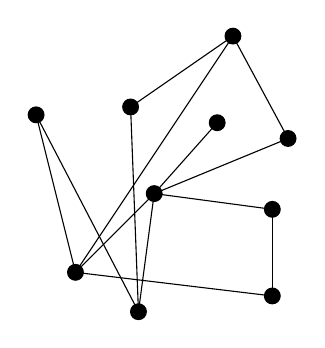
\begin{tikzpicture}
  \node[circle,draw,fill=black,minimum size=2mm,inner sep=0pt,outer sep=0pt]
  (v1) at (0, 0) {};
  \node[circle,draw,fill=black,minimum size=2mm,inner sep=0pt,outer sep=0pt]
  (v2) at (1, 2) {};
  \node[circle,draw,fill=black,minimum size=2mm,inner sep=0pt,outer sep=0pt]
  (v3) at (-1, -1) {};
  \node[circle,draw,fill=black,minimum size=2mm,inner sep=0pt,outer sep=0pt]
  (v4) at (-1.5, 1) {};
  \node[circle,draw,fill=black,minimum size=2mm,inner sep=0pt,outer sep=0pt]
  (v5) at (1.5, -1.3) {};
  \node[circle,draw,fill=black,minimum size=2mm,inner sep=0pt,outer sep=0pt]
  (v6) at (1.7, 0.7) {};
  \node[circle,draw,fill=black,minimum size=2mm,inner sep=0pt,outer sep=0pt]
  (v7) at (-0.2, -1.5) {};
  \node[circle,draw,fill=black,minimum size=2mm,inner sep=0pt,outer sep=0pt]
  (v8) at (0.8, 0.9) {};
  \node[circle,draw,fill=black,minimum size=2mm,inner sep=0pt,outer sep=0pt]
  (v9) at (-0.3, 1.1) {};
  \node[circle,draw,fill=black,minimum size=2mm,inner sep=0pt,outer sep=0pt]
  (v10) at (1.5, -0.2) {};

  \draw (v1) -- (v3);
  \draw (v1) -- (v6);
  \draw (v1) -- (v7);
  \draw (v1) -- (v8);
  \draw (v1) -- (v10);
  \draw (v2) -- (v3);
  \draw (v2) -- (v6);
  \draw (v2) -- (v9);
  \draw (v3) -- (v4);
  \draw (v3) -- (v5);
  \draw (v4) -- (v7);
  \draw (v5) -- (v10);
  \draw (v7) -- (v9);
 \end{tikzpicture}
 \caption{Náhodný graf na deseti vrcholech.}
 \label{fig:random-graph-on-10-pts}
\end{figure}

Otázka, kterou se budeme časem zabývat zní \uv{Kolik maximálně mohu nakreslit
spojnic, než mi vznikne trojúhelník?} Trojúhelníkem zde myslíme trojici bodů,
z nichž každé dva jsou spojeny. Do tohoto grafu se určitě ještě dají nějaké
přikreslit, ale kolik přesně? A jak tuto úlohu řešit obecně pro jakýkoliv
počet bodů?

Podobně zajímavá, ale už víc algoritmická otázka, by zněla \uv{Jak poznám,
jestli v nějakém grafu existuje trojúhelník?}. Samozřejmě by šlo se prostě
podívat na každou jednu trojici bodů, ale jde to i líp?

Ještě na pár odstavců zůstaneme u spojených puntíků. Úloha, která se ukázala
jako zásadní v teorii grafů má co dělat s cestami. \emph{Cestou} v grafu
nazveme posloupnost bodů -- vrcholů, takovou, že mezi sousedními vrcholy na
cestě vždycky vede spojnice. Jinak řečeno, mohu se v klidu projít od jednoho
vrcholu k druhému, aniž bych musel skákat mezi vrcholy. Naším úkolem je najít
takovou množinu spojnic -- hran, že se mezi každými dvěma vrcholy dá projít po
cestě.

Pro deset vrcholů jedno možné řešení vidíte na
\hyperref[fig:minimal-skeleton-on-10-pts]{obrázku
\ref*{fig:minimal-skeleton-on-10-pts}}.

\begin{figure}[h]
 \centering
 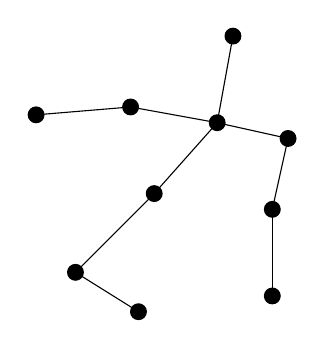
\begin{tikzpicture}
  \node[circle,draw,fill=black,minimum size=2mm,inner sep=0pt,outer sep=0pt]
  (v1) at (0, 0) {};
  \node[circle,draw,fill=black,minimum size=2mm,inner sep=0pt,outer sep=0pt]
  (v2) at (1, 2) {};
  \node[circle,draw,fill=black,minimum size=2mm,inner sep=0pt,outer sep=0pt]
  (v3) at (-1, -1) {};
  \node[circle,draw,fill=black,minimum size=2mm,inner sep=0pt,outer sep=0pt]
  (v4) at (-1.5, 1) {};
  \node[circle,draw,fill=black,minimum size=2mm,inner sep=0pt,outer sep=0pt]
  (v5) at (1.5, -1.3) {};
  \node[circle,draw,fill=black,minimum size=2mm,inner sep=0pt,outer sep=0pt]
  (v6) at (1.7, 0.7) {};
  \node[circle,draw,fill=black,minimum size=2mm,inner sep=0pt,outer sep=0pt]
  (v7) at (-0.2, -1.5) {};
  \node[circle,draw,fill=black,minimum size=2mm,inner sep=0pt,outer sep=0pt]
  (v8) at (0.8, 0.9) {};
  \node[circle,draw,fill=black,minimum size=2mm,inner sep=0pt,outer sep=0pt]
  (v9) at (-0.3, 1.1) {};
  \node[circle,draw,fill=black,minimum size=2mm,inner sep=0pt,outer sep=0pt]
  (v10) at (1.5, -0.2) {};
  
  \draw (v4) -- (v9);
  \draw (v9) -- (v8);
  \draw (v8) -- (v2);
  \draw (v8) -- (v6);
  \draw (v8) -- (v1);
  \draw (v1) -- (v3);
  \draw (v3) -- (v7);
  \draw (v6) -- (v10);
  \draw (v10) -- (v5);
 \end{tikzpicture}
 \caption{Minimální kostra grafu na deseti vrcholech.}
 \label{fig:minimal-skeleton-on-10-pts}
\end{figure}

Je jednoduché si rozmyslet, kolik nejméně hran je třeba nakreslit. Ovšem, co
když můžeme vybírat jen z nějaké předem dané množiny? Řešení pak nemusí vždycky
existovat (může se totiž stát, že žádné hrany k dispozici nemáme). Dá se nějak
efektivně poznat, kdy úlohu lze řešit a kdy ne? A co třeba otázka, kolik
existuje řešení s minimálním počtem hran; co řešení, součet přes všechny jehož
hrany je nejmenší? V této obecné podobě se úloze (i jejímu řešení) říká
\emph{minimální kostra} grafu a v budoucnu ji, stejně jako předchozí dvě úlohy,
potkáme.
